\documentclass[10pt]{article}

% Pacotes extras necessários
\usepackage{amsmath}
\usepackage[lmargin=0.5in, rmargin=0.5in, tmargin=0.5in, bmargin=0.5in, includehead, includefoot]{geometry}
\usepackage{amsfonts}
\usepackage[utf8]{inputenc}
\usepackage[portuguese]{babel}
\usepackage{graphicx}
\usepackage{fancyhdr}
\usepackage{setspace}
\usepackage{listings}
\usepackage{url}
\usepackage{enumitem}
\usepackage{appendix} % For creating appendix sections

% More defined colors
\usepackage[dvipsnames]{xcolor}

% Define a custom style for the code listing
\lstdefinestyle{mystyle}{
    language=Octave,
    backgroundcolor=\color{white},   % Choose the background color
    basicstyle=\ttfamily\footnotesize, % Set the font and size for the code
    numbers=left,                    % Line numbers on the left
    numberstyle=\tiny\color{gray},   % Line numbers style
    numbersep=5pt,                   % Distance of line numbers from the code
    tabsize=2,                       % Set tab size (default is 8 spaces)
    breaklines=true,                 % Automatically wrap long lines
    keywordstyle=\color{blue},       % Keywords in blue
    commentstyle=\color{green!60!black}, % Comments in green
    stringstyle=\color{orange},      % Strings in orange
    frame=single,                    % Draw a frame around the code
    keepspaces=true,                 % Preserve spaces in text
    showspaces=false,                % Don't show spaces in strings
    showstringspaces=false,          % Don't show spaces in strings
    showtabs=false,                  % Don't show tabs in strings
    % Add any other options you need
}

\lstset{style=mystyle} % Set the custom style
 
% Required package
\usepackage{tikz}
\usetikzlibrary{positioning}

\graphicspath{ {./images/} }

% Sets para outras partes
\setlength{\parindent}{0pt}
\setstretch{1.5}
\DeclareMathOperator{\sen}{sen}
\DeclareMathOperator{\sinc}{sinc}

%% Facilidades
%% -- Laplace
\newcommand{\Lap}[1]{\mathcal{L}\left\{#1\right\}}

%% -- Negrito em matemáticas
\newcommand{\bm}[1]{\boldsymbol{#1}}


% ------- Estilo do trabalho -------- %
\fancypagestyle{capa}{
    \fancyhf{}
    \renewcommand\headrulewidth{0pt}
}

\pagestyle{fancy}
\fancyhead{}
\fancyhead[L]{\thepage}
\fancyfoot{}
% ----------------------------------- %

% Dados do Grupo
\title{Modelagem de Sistemas Dinâmicos - Trabalho Nº4}
\author{
    Leonardo Soares da Costa Tanaka - DRE: 121067652 \\
    Engenharia de Controle e Automação/UFRJ \\
    Rio de Janeiro, Brasil \\
    Julho de 2023
}
\date{}

\begin{document}
\maketitle
\thispagestyle{capa}

\quad Para este trabalho, vamos utilizar o arquivo “trabalho4-2023-1.mat” que tem os sinais de entrada u(t) e de saída y(t) de um sistema
linear contínuo com função de transferência G(s). Os sinais u e y foram aplicados e aquisitados
com uma frequência de amostragem fs = 2Hz (período de amostragem T = 0.5s). A variável
independente tempo t é o vetor com os instantes que foram realizadas as amostragens dos
sinais u(t) e y(t).

\quad Vale notar que o sinal de saída y(t) está quantizado e contaminado com ruído.

\section{FFT}

\quad Determinando, utilizando a FFT (Fast Fourier Transform), o espectro do sinal de entrada
(módulo e fase) em função da frequência em Hz. Utilizando o Matlab para coletar os dados,
utilizar a FFT, calcular os espectros do sinal de entrada e plotar o gráfico.

\begin{figure}[h]
    \centering
    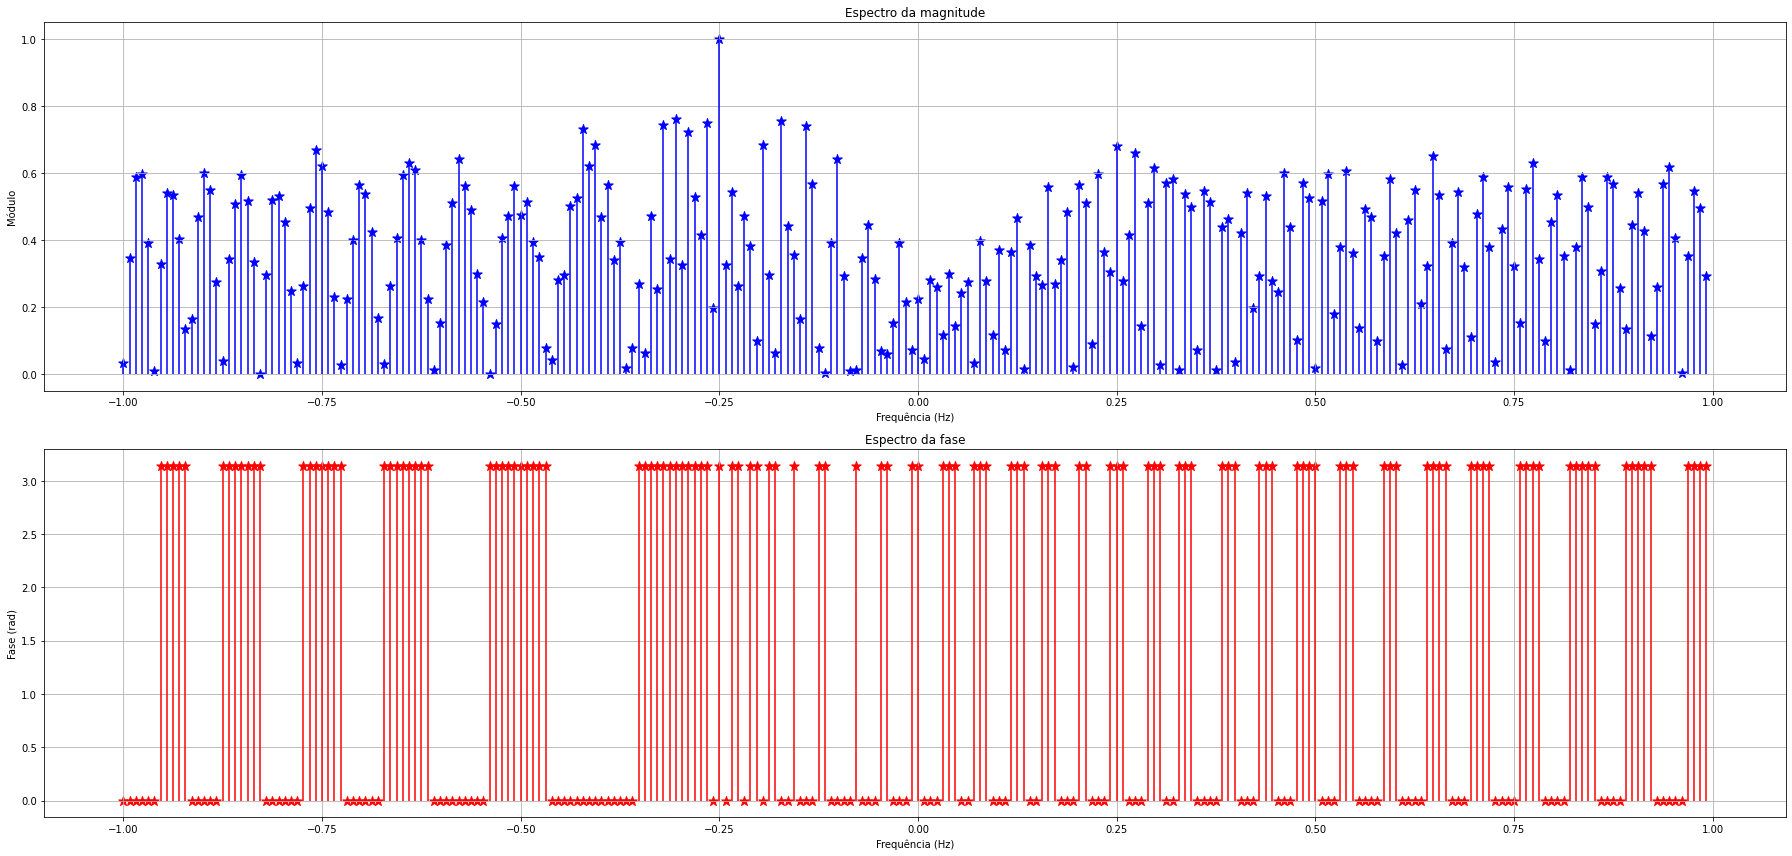
\includegraphics[scale=0.34]{fft.png}
    \caption{Espectros dos sinais da entrada}
\end{figure}

\quad É possível observar uma simetria no gráfico da mangnitude em torno de 1
com uma parte central com valores iguais a 2.61115 entre 0.4 e 1.6,
duas partes seguintes com valores iguais a 10.4446 entre (0.03 e 0.4) e (1.6 e 1.96) e duas
partes extremas com os mesmos valores que a parte central. Já no gráfico de fase, é possível
observar uma oscilação bem similar entre 0.4 e 1.6 e
outras oscilações similares entre (0.03 e 0.4) e (1.6 e 1.96) com valores entre $-\pi$ e $\pi$.

\section{Resposta em frequência do sistema G(jw)}

\quad Estimando a resposta em frequência do sistema G(jw) utilizando os espectros dos sinais
de entrada U(jw) e de saída Y(jw):

\begin{figure}[h]
    \centering
    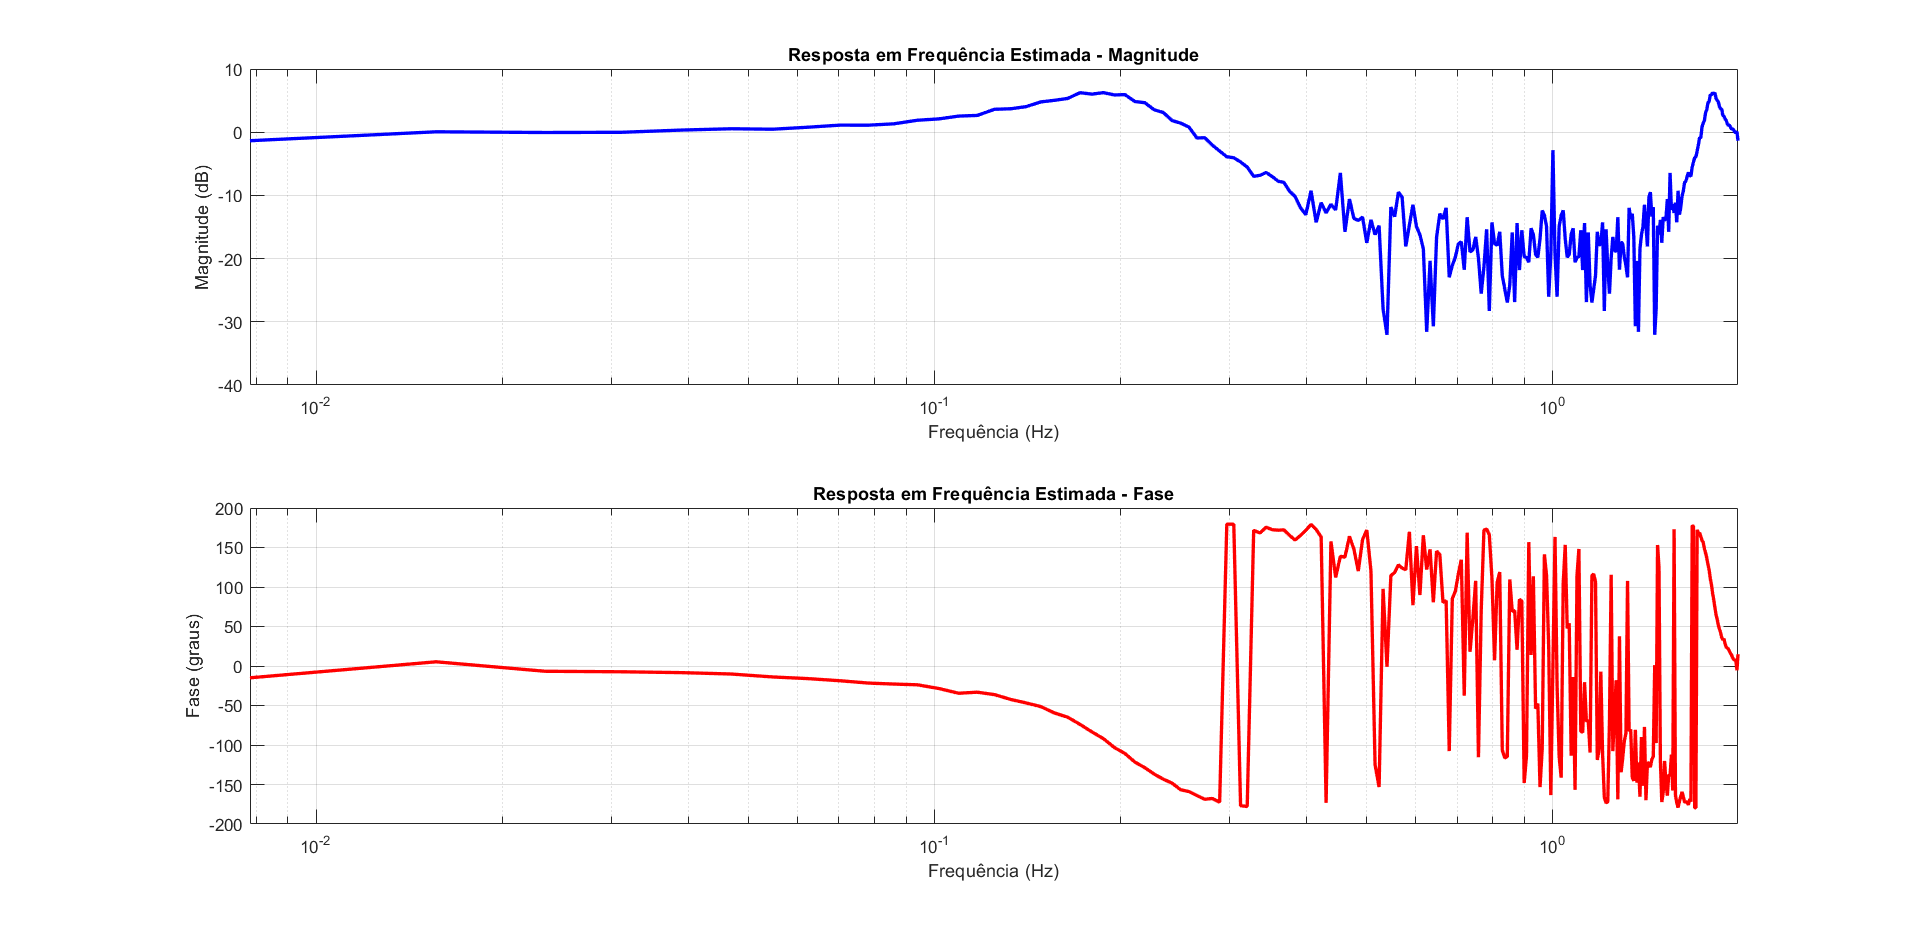
\includegraphics[scale=0.34]{g.png}
    \caption{Resposta em frequência do sistema G(jw)}
\end{figure}

\section{Principais caracteríticas da resposta em frequência}

\newpage

\section{Determinação do sistema de $2\textsuperscript{a}$ ordem}

\quad Para determinar o sistema de $2\textsuperscript{a}$ ordem que tem resposta em frequência mais próxima com a estimada,
foi feito diversos testes trocando as constantes $\zeta$ e $w_n$
até chegar numa visualização bem próxima entre as duas respostas em frequência.

\begin{figure}[h]
    \centering
    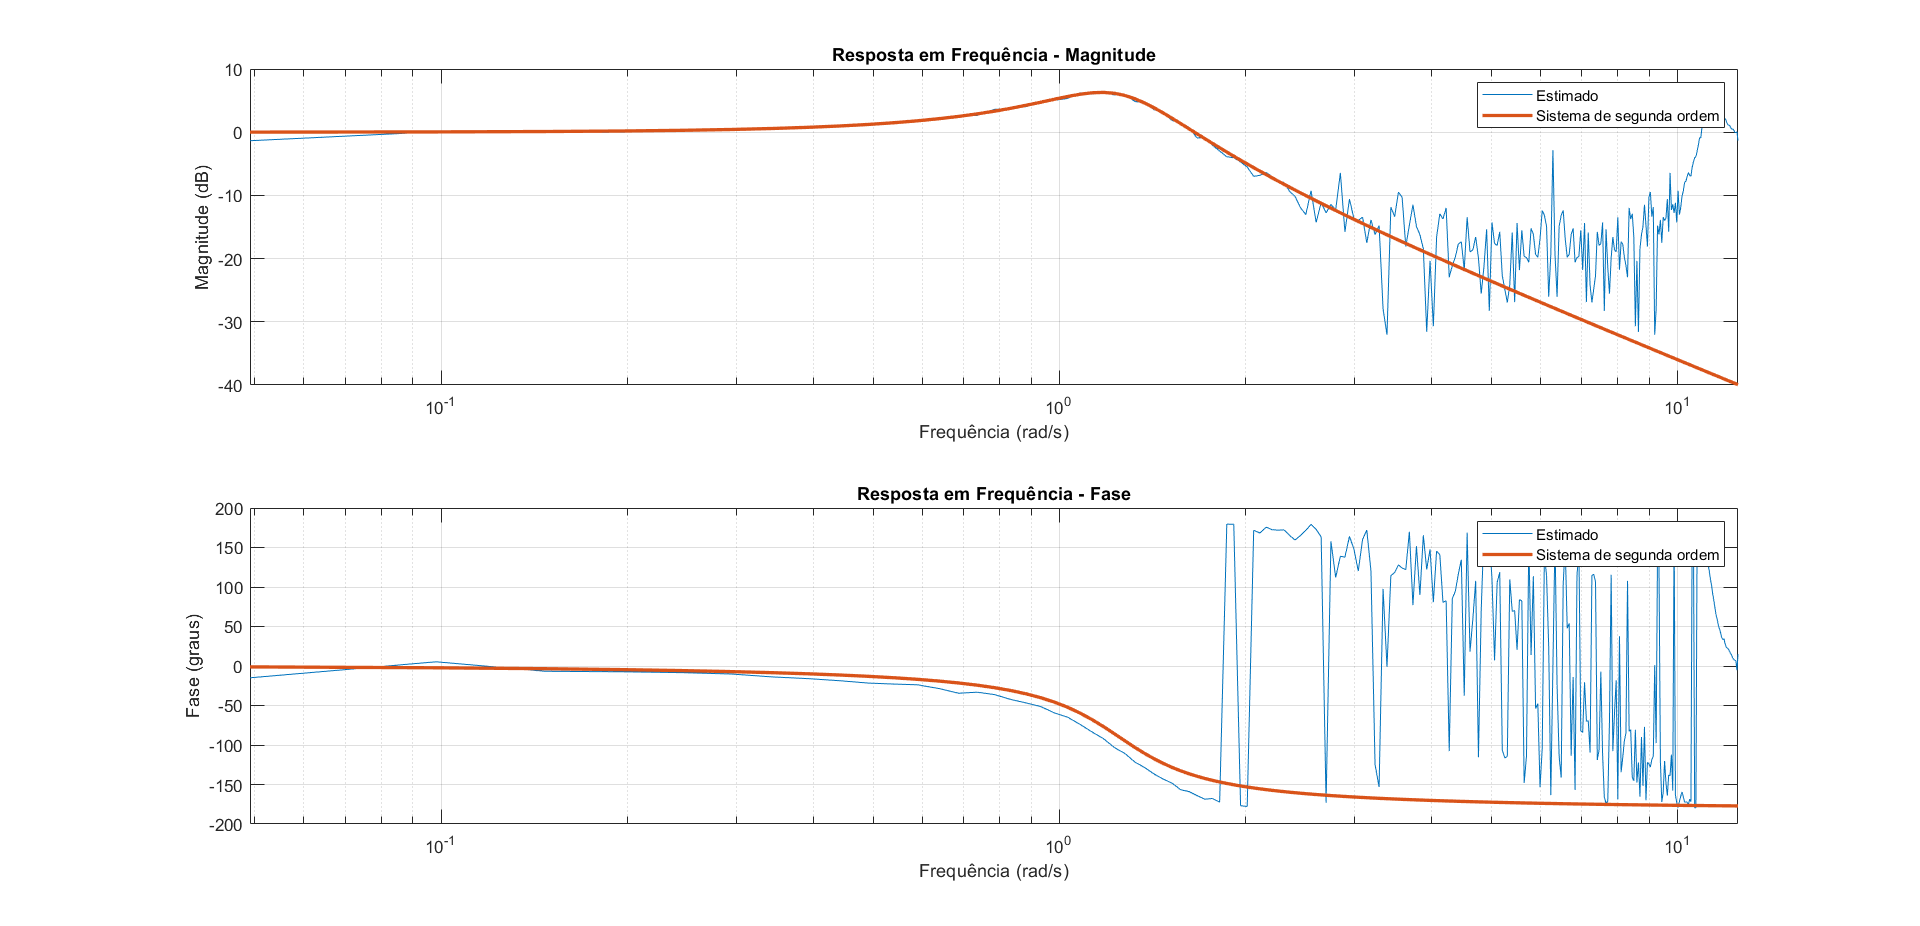
\includegraphics[scale=0.35]{g_manual.png}
    \caption{Resposta em frequência}
\end{figure}

\quad Foi utilizada a seguinte fórmula que representa a função de transferência de um sistema de $2\textsuperscript{a}$ ordem:

\begin{equation}
    G(s) = \frac{\omega_n^2}{s^2 + 2 \zeta \cdot \omega_n \cdot s + \omega_n^2}
\end{equation}

\quad Os valores obtidos foram:

\begin{equation}
    w_n = 0.2 \ e \ \zeta = 0.25
\end{equation}

\newpage

\section{System Identification Apps}

\begin{figure}[h]
    \centering
    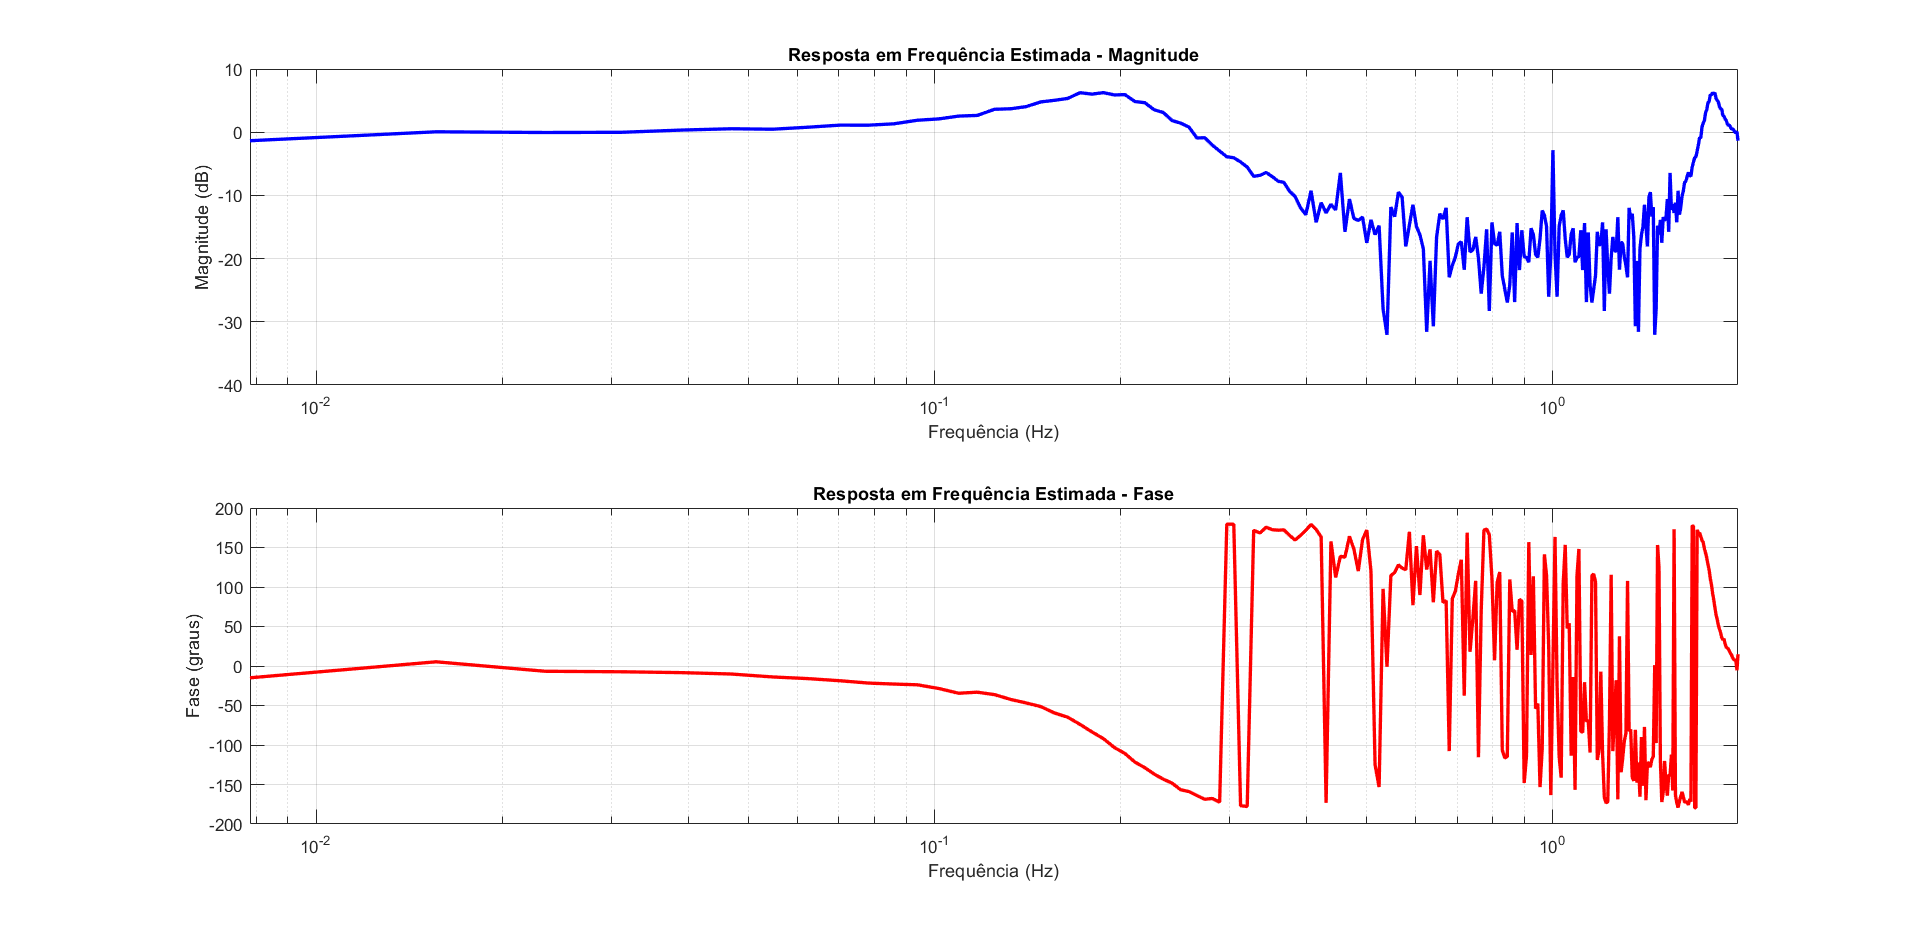
\includegraphics[scale=0.2]{g.png}
    \caption{Resposta em frequência do sistema G(jw)}
\end{figure}

\begin{figure}[h]
    \centering
    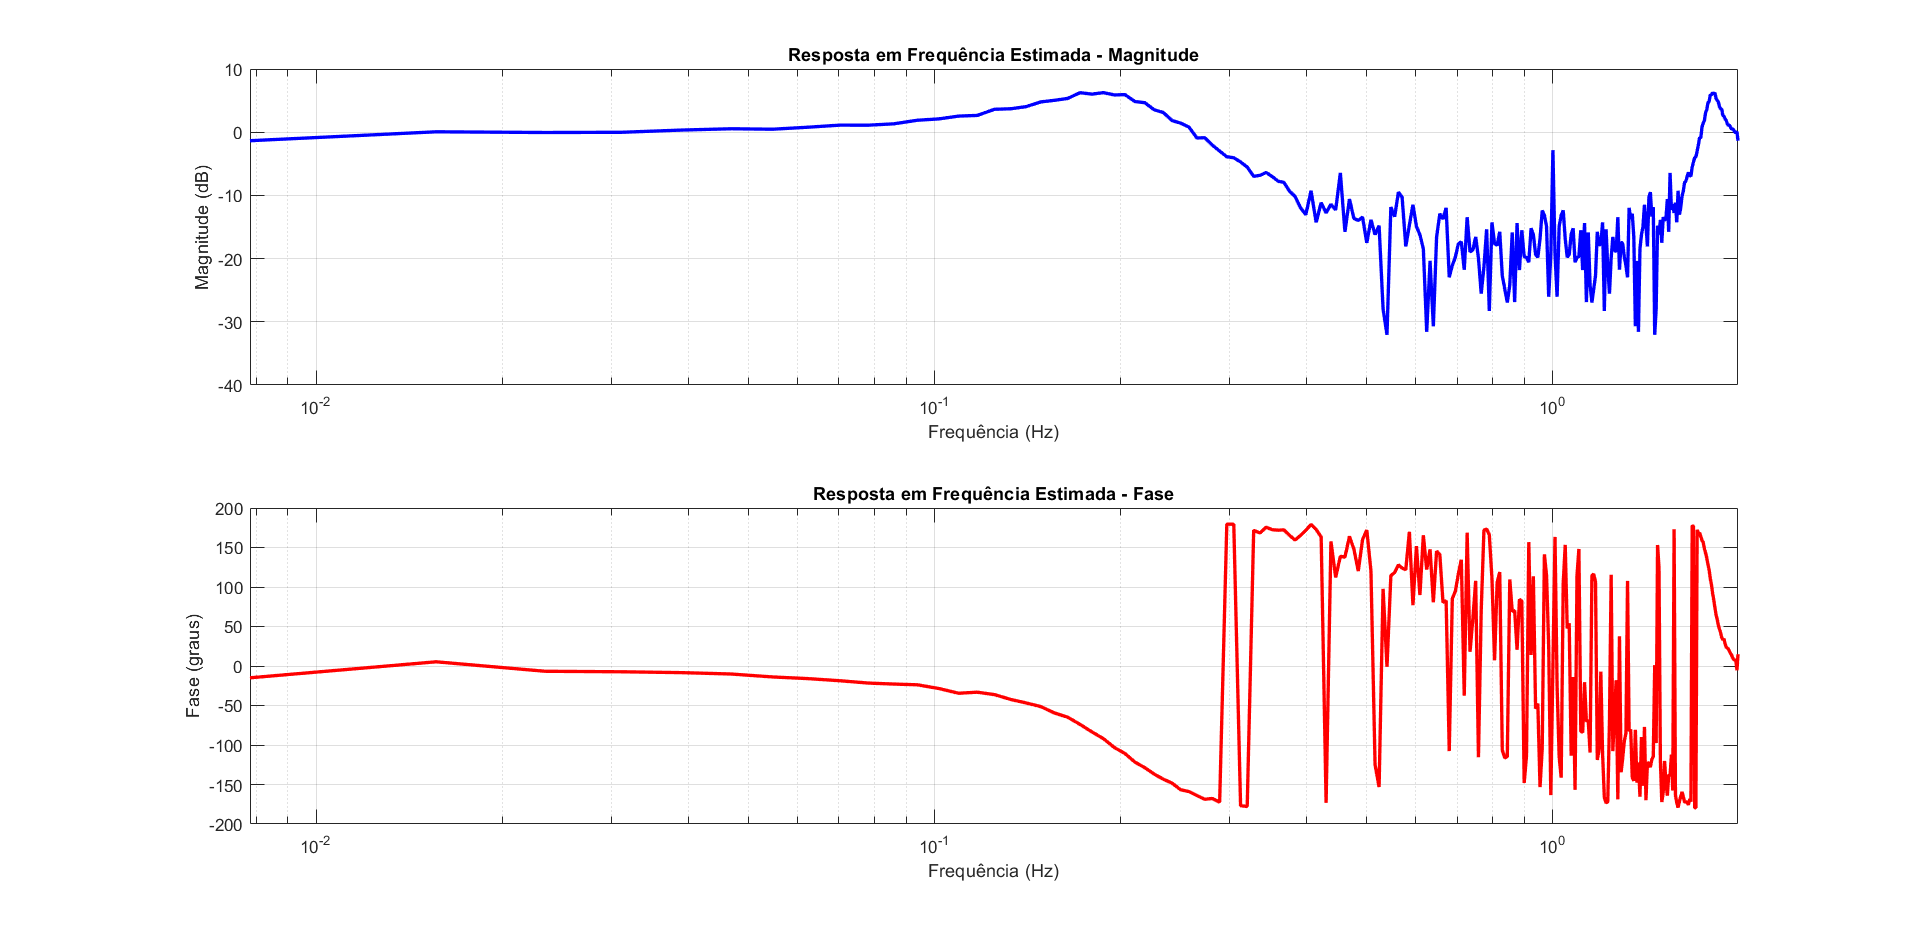
\includegraphics[scale=0.2]{g.png}
    \caption{Resposta em frequência do sistema G(jw)}
\end{figure}

\begin{figure}[h]
    \centering
    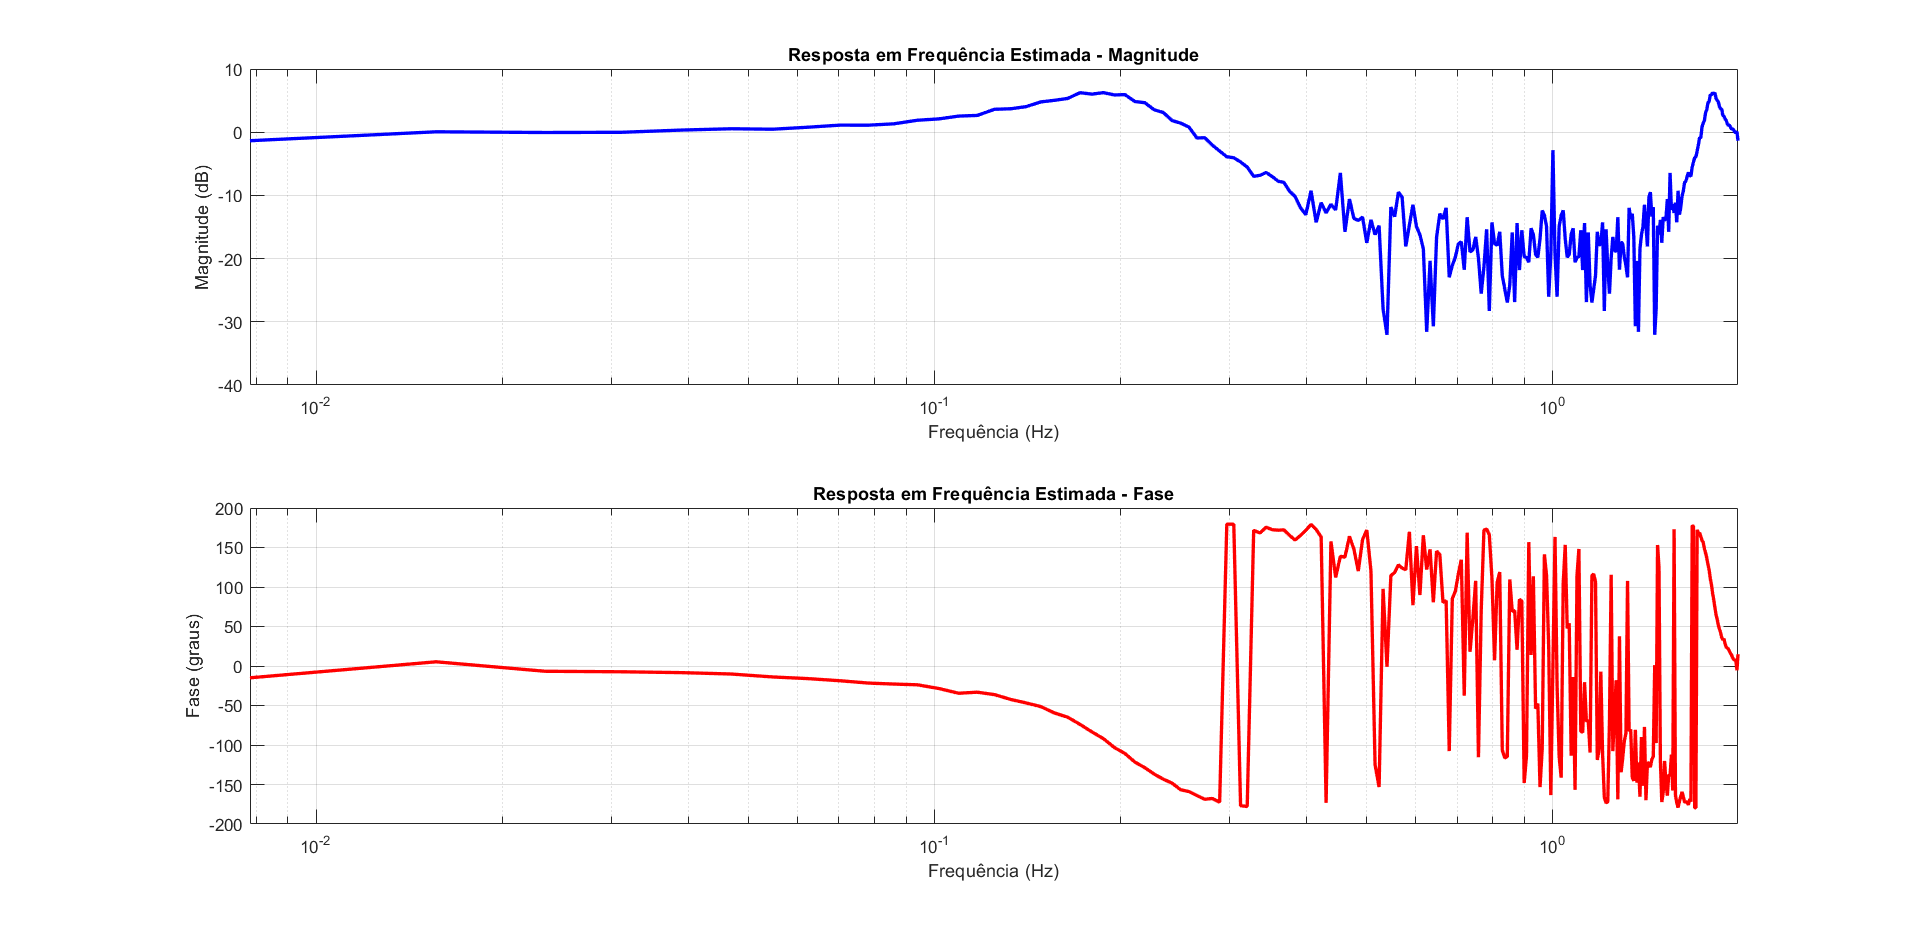
\includegraphics[scale=0.2]{g.png}
    \caption{Resposta em frequência do sistema G(jw)}
\end{figure}

\newpage

\begin{appendices}

\section{Código 1}

\begin{verbatim}
    data = load('trabalho4-2023-1.mat'); % Carregar os dados do arquivo
    u = data.u;
    t = data.t;
    fs = 2; % Hz % Frequência de amostragem (fs) e período de amostragem (T)
    T = 1 / fs;
    U = fft(u); % Calcula o espectro do sinal de entrada u(t) usando a FFT
    frequencies = (0:length(U) - 1) * (fs / length(U)); % Vetor de frequências para o eixo x
    modulo_U = abs(U); % Módulo do espectro do sinal de entrada
    fase_U = angle(U); % Fase do espectro do sinal de entrada
    % Cores para os plots
    cor_modulo = 'b'; % Azul
    cor_fase = 'r';   % Vermelho
    figure; % Plot do espectro do sinal de entrada (módulo e fase)
    subplot(2, 1, 1); % Plot do módulo do espectro
    stem(frequencies, modulo_U, 'Color', cor_modulo);
    xlabel('Frequência (Hz)');
    ylabel('Módulo');
    title('Módulo do espectro do Sinal de Entrada u(t)');
    grid on;
    subplot(2, 1, 2); % Plot da fase do espectro
    stem(frequencies, fase_U, 'Color', cor_fase);
    xlabel('Frequência (Hz)');
    ylabel('Fase (rad)');
    title('Fase do Espectro do Sinal de Entrada u(t)');
    grid on;
\end{verbatim}

\newpage

\section{Código 2}

\begin{verbatim}
    load('trabalho4-2023-1.mat'); % Carregar o arquivo 'trabalho4-2023-1.mat'
    fs = 2; % Hz % Frequência de amostragem
    U = fft(u); % Realizar a FFT do sinal de entrada 'u'
    Y = fft(y); % Realizar a FFT do sinal de saída 'y'
    G_estimated = Y ./ U; % Estimar a resposta em frequência do sistema G(jw)
    G_mag_dB = 20*log10(abs(G_estimated));
    G_phase_deg = rad2deg(angle(G_estimated));
    N = length(u);
    frequencies = (0:N-1) * (fs/N); % Frequências correspondentes
    figure; % Plotar o módulo e fase da resposta em frequência estimada na mesma figura em escala logarítmica
    subplot(2, 1, 1);
    semilogx(frequencies, G_mag_dB, 'b', 'LineWidth', 2);
    title('Resposta em Frequência Estimada - Magnitude');
    xlabel('Frequência (Hz)');
    ylabel('Magnitude (dB)');
    grid on;
    subplot(2, 1, 2);
    semilogx(frequencies, G_phase_deg, 'r', 'LineWidth', 2);
    title('Resposta em Frequência Estimada - Fase');
    xlabel('Frequência (Hz)');
    ylabel('Fase (graus)');
    grid on; 
\end{verbatim}

\newpage

\section{Código 4}

\begin{verbatim}
    load('trabalho4-2023-1.mat'); % Carregamento dos dados (substitua 'trabalho4-2023-1.mat' pelo nome correto do arquivo)
    fs = 2; % Frequência de amostragem em Hz 
    freq = (0:length(u)-1) * fs / length(u); % Vetor de frequências em Hz
    U = fft(u); % Cálculo do espectro de entrada e saída
    Y = fft(y);
    H_estimado = Y ./ U; % Estimativa da resposta em frequência
    % Inicialização dos parâmetros para ajuste manual
    wn_guess = 0.2;
    zeta_guess = 0.25;
    % Calcula a resposta em frequência para os valores iniciais dos parâmetros
    sistema = tf(wn_guess^2, [1, 2 * zeta_guess * wn_guess, wn_guess^2]);
    H_modelo = freqresp(sistema, freq);
    figure; % Plota a resposta em frequência estimada e do modelo inicial (magnitude)
    subplot(2, 1, 1);
    semilogx(freq, 20 * log10(abs(H_estimado)), 'b', 'LineWidth', 2);
    hold on;
    semilogx(freq, 20 * log10(abs(squeeze(H_modelo))), 'r', 'LineWidth', 2);
    xlabel('Frequência (Hz)');
    ylabel('Magnitude (dB)');
    legend('Estimado', 'Modelo');
    grid on;
    subplot(2, 1, 2); % Plota a resposta em frequência do modelo inicial (fase em graus)
    semilogx(freq, rad2deg(angle(H_estimado)), 'b', 'LineWidth', 2);
    hold on;
    semilogx(freq, rad2deg(angle(squeeze(H_modelo))), 'r', 'LineWidth', 2);
    xlabel('Frequência (Hz)');
    ylabel('Fase (graus)');
    legend('Estimado', 'Modelo');
    grid on;
\end{verbatim}

\end{appendices}

\end{document}